\scanpage{24}
% letterhead
\begin{center}
I N S T I T U T\\
DES HAUTES ÉTUDES SCIENTIFIQUES\\
\rule{1cm}{0.4pt}
\end{center}

\handwritten{SGA 4 $\overline{\text{\uline{VII}}}$\quad p. 20}

\handwritten{\uline{Ajouter} 5.6. \textcircled{a} $\tilde{X}_{\mathrm{et}}$ est
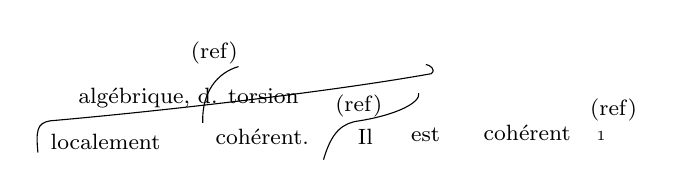
\begin{tikzpicture}[x=.013cm,y=-.013cm,baseline=(localement.base),every node/.style={anchor=base west,inner sep=0pt,font=\footnotesize}]
\path[use as bounding box] (429,244) rectangle (1055,380);
\node (localement) at (451,363) {localement};
\node at (612,358) {cohérent.};
\node at (751,358) {Il};
\node at (803,355) {est};
\node at (874,354) {cohérent};
\node[font=\tiny] at (984,354) {\deleted{\illegible{1}}};
\node at (478,318) {\inserted{algébrique, d. torsion}};
\node at (588,274) {\inserted{(ref)}};
\node at (729,326) {\inserted{(ref)}};
\node at (978,330) {\inserted{(ref)}};
\draw[line width=.4pt] (439,366) .. controls (437,345) and (438,337) .. (451,335) .. controls (565,325) and (728,306) .. (823,289) .. controls (829,285) and (821,280) .. (818,280);
\draw[line width=.4pt] (600,337) .. controls (599,307) and (614,288) .. (635,282);
\draw[line width=.4pt] (718,373) .. controls (726,345) and (737,337) .. (753,335) .. controls (790,329) and (813,317) .. (811,308);
\end{tikzpicture}
(resp. quasi-séparé\inserted{(ref)}) \deleted{\illegible{1}} sss le schéma $X$ est \deleted{\unsure{quasi-cpt}} cohérent i.e. qu. cpt qu. sép (resp. quasi-séparé). \deleted{\illegible{1}}}

\handwritten{\textcircled{b} Soit $(X_i)_{i\in I}$ système projectif filtrant à morphismes de transition affines, $X=\varprojlim_i X_i$ (EGA $\overline{\text{\uline{IV}}}$ 8),}

\handwritten{Âlors}
\[
\handwritten{\tilde{X}_{\mathrm{et}}\simeq\underset{\longleftarrow}{\mathrm{limtop}}\,\tilde{X}_i.}
\]

\handwritten{En \unsure{deduire|déduire} pour 5.7.}

\margin{\hspace*{-3.1cm}\handwritten{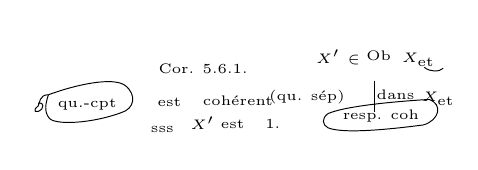
\begin{tikzpicture}[x=.012cm,y=-.012cm,every node/.style={anchor=base west,inner sep=0pt,font=\tiny}]
\path[use as bounding box] (628,662) rectangle (1075,783);
\node at (766,711) {\uline{Cor.} 5.6.1.};
\node at (933,700) {$X'$};
\node at (966,700) {$\in$};
\node at (986,697) {$\mathrm{Ob}$};
\node at (1024,699) {$X_{\mathrm{et}}$};
\draw[line width=.35pt] (1048,704) .. controls (1054,709) and (1064,709) .. (1068,705);
\node at (765,746) {est};
\node at (813,744) {\deleted{\unsure{cohérent}}};
\node at (883,739) {(\unsure{qu. sép})};
\node at (997,738) {dans};
\node at (1045,740) {$X_{\mathrm{et}}$};
\node at (758,773) {sss};
\node at (800,770) {$X'$};
\node at (832,769) {est};
\node at (879,769) {\deleted{\illegible{1}}.};
\node[anchor=center] at (691,743) {\inserted{\unsure{qu.-cpt}}};
\draw[line width=.35pt] (650,733) .. controls (680,722) and (718,714) .. (731,723) .. controls (744,733) and (741,748) .. (727,752) .. controls (694,764) and (657,765) .. (651,758) .. controls (645,751) and (647,742) .. (650,733);
\draw[line width=.35pt] (650,733) .. controls (640,733) and (641,742) .. (639,745) .. controls (632,750) and (637,754) .. (643,748) .. controls (646,743) and (642,741) .. (639,742);
\node[anchor=center] at (1002,756) {\inserted{resp. coh}};
\draw[line width=.35pt] (995,718) -- (995,751);
\draw[line width=.35pt] (946,753) .. controls (964,745) and (1018,740) .. (1053,738) .. controls (1068,743) and (1064,760) .. (1047,765) .. controls (1016,769) and (963,775) .. (946,768) .. controls (940,765) and (939,758) .. (946,753);
\end{tikzpicture}}}

\figure{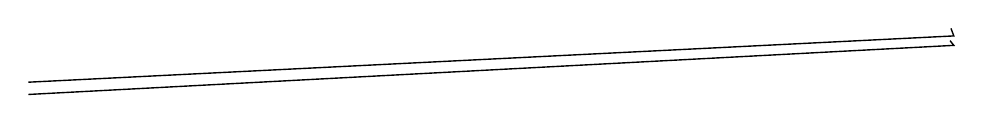
\begin{tikzpicture}[x=.012cm,y=.012cm]
\draw[line width=.5pt] (0,0) -- (980,49) -- (977,57);
\draw[line width=.5pt] (0,-13) -- (980,39) -- (976,44);
\end{tikzpicture}}

\handwritten{SGA 4 $\overline{\text{\uline{IX}}}$\quad p. 42\qquad note \uline{pour} la p. 8}

\figure{\begin{tikzpicture}[x=.012cm,y=.012cm]
\draw[line width=.4pt] (0,0) .. controls (290,19) and (660,57) .. (999,67);
\end{tikzpicture}}

\handwritten{$\overline{\text{\uline{VII}}}$\quad 2.1 c)\qquad (p. 9)\quad \uline{corriger}}
% archive sheet number: 23
